% ==============================================================================
% SECAO 3 — MODELAGEM MATEMATICA E MALHA ABERTA
% ==============================================================================
\section{MAPEAMENTO MATEMÁTICO E DINÂMICA EM MALHA ABERTA}\label{sec:malha_aberta}

Esta seção combina as duas equações de primeira ordem da Seção~\ref{sec:modelagem_fisica} em um modelo único da planta e analisa seu comportamento sem realimentação.

\subsection{Equação Diferencial de Segunda Ordem da Planta}\label{sec:edo_planta}
Sob taxa de chegada nominal ($\lambda(t) = 1000\text{ eventos/s}$, logo $\Delta\lambda(t) = 0$), a Equação~\eqref{eq:balanco_x} fornece $\Delta\mu(t) = \dot{x}(t)$ e, por derivação temporal, $\Delta\dot{\mu}(t) = \ddot{x}(t)$. Substituindo ambas as relações na Equação~\eqref{eq:atuador_inc}, obtém-se a EDO linear de segunda ordem que relaciona a redução da fila $x(t)$ ao incremento de capacidade solicitado $u(t)$:
\begin{equation}
    2\,\frac{d^2 x(t)}{dt^2} + \frac{dx(t)}{dt} = u(t), \qquad x(0) = 0,\quad \dot{x}(0) = 0.
    \label{eq:edo_2ordem}
\end{equation}
De forma mais geral, na presença de variação de chegada $\Delta\lambda(t)$, a dinâmica acoplada satisfaz $2\ddot{x}(t) + \dot{x}(t) = u(t) - 2\Delta\dot{\lambda}(t) - \Delta\lambda(t)$.

\subsection{Função de Transferência em Malha Aberta e Resposta ao Degrau}\label{sec:ft_ma}
Aplicando a transformada de Laplace à Equação~\eqref{eq:edo_2ordem} com condições iniciais incrementais nulas ($x(0)=0, \dot{x}(0)=0$), obtém-se a função de transferência em malha aberta (NISE, 2017):
\begin{equation}
    (2s^2 + s)X(s) = U(s) \implies G(s) = \frac{X(s)}{U(s)} = \frac{1}{s(2s + 1)} = \frac{0{,}5}{s(s + 0{,}5)}.
    \label{eq:ft_planta}
\end{equation}

Do ponto de vista modal e estrutural, a função $G(s)$ não apresenta zeros finitos, exibindo grau relativo igual a $2$ (com dois zeros no infinito). Seus polos situam-se sobre o eixo real em $p_1 = 0$, que confere à planta natureza integradora pura e a classifica como um sistema de \textit{Tipo~1}, e em $p_2 = -0{,}5\text{ s}^{-1}$, modo exponencial decrescente diretamente associado à constante de tempo $\tau = 2\text{ s}$ da infraestrutura computacional. Pelo fato de possuir um polo na origem e carecer de termo restaurador de ordem zero no denominador ($s^2 + 0{,}5s + 0$), a forma canônica de segunda ordem não se aplica, pois $\omega_n = 0$ e a identidade $2\zeta\omega_n = 0{,}5$ só seria satisfeita no limite $\zeta \to \infty$.

Consequentemente, em malha aberta, a planta é classificada como marginalmente estável (e, portanto, não BIBO-estável, pois uma entrada limitada em degrau produz saída em rampa), integradora e não oscilatória. Submetendo-a a uma entrada em degrau $u(t) = U_0\,\mathbb{1}(t)$, isto é, $U(s) = U_0/s$, obtém-se a resposta no domínio da frequência e no tempo:
\begin{equation}
    X(s) = \frac{U_0}{s^2(2s + 1)} = U_0\left(\frac{1}{s^2} - \frac{2}{s} + \frac{2}{s + 0{,}5}\right)
    \implies x(t) = U_0\left(t - 2 + 2e^{-0{,}5t}\right)\mathbb{1}(t).
    \label{eq:resp_degrau_ma}
\end{equation}
A Equação~\eqref{eq:resp_degrau_ma} revela que $x(t)$ cresce indefinidamente segundo uma rampa assintótica $x(t) \approx U_0(t - 2)$, com inclinação igual a $U_0$~eventos/s e atraso efetivo de $\tau = 2\text{ s}$ após o transiente exponencial, conforme ilustra a Figura~\ref{fig:malha_aberta}. Do ponto de vista físico, qualquer excesso constante de capacidade ($U_0 > 0$) drena continuamente o estoque acumulado até a exaustão física da fila em $q(t) = 0$ ($x(t) = 600$~eventos). Na simulação numérica, o esvaziamento ocorre em $t = 7{,}97\text{ s}$ para $U_0 = 100$~eventos/s (com $\mu \to 1099{,}75$~eventos/s) e em $t = 3{,}69\text{ s}$ para $U_0 = 300$~eventos/s ($\mu \to 1299{,}26$~eventos/s), demonstrando a impossibilidade de regular a fila em um patamar finito ($q_r = 300$~eventos) sem realimentação corretiva.

\begin{figure}[H]
    \centering
    \caption{Resposta em malha aberta da redução da fila $x(t)$, da fila real $q(t)$ e da capacidade efetiva $\mu(t)$ para degraus incrementais $U_0 = 100$ e $300\text{ eventos/s}$, evidenciando a rampa assintótica até o esvaziamento físico $q(t)=0$}
    \label{fig:malha_aberta}
    \IfFileExists{figuras/fig1_malha_aberta.pdf}{%
        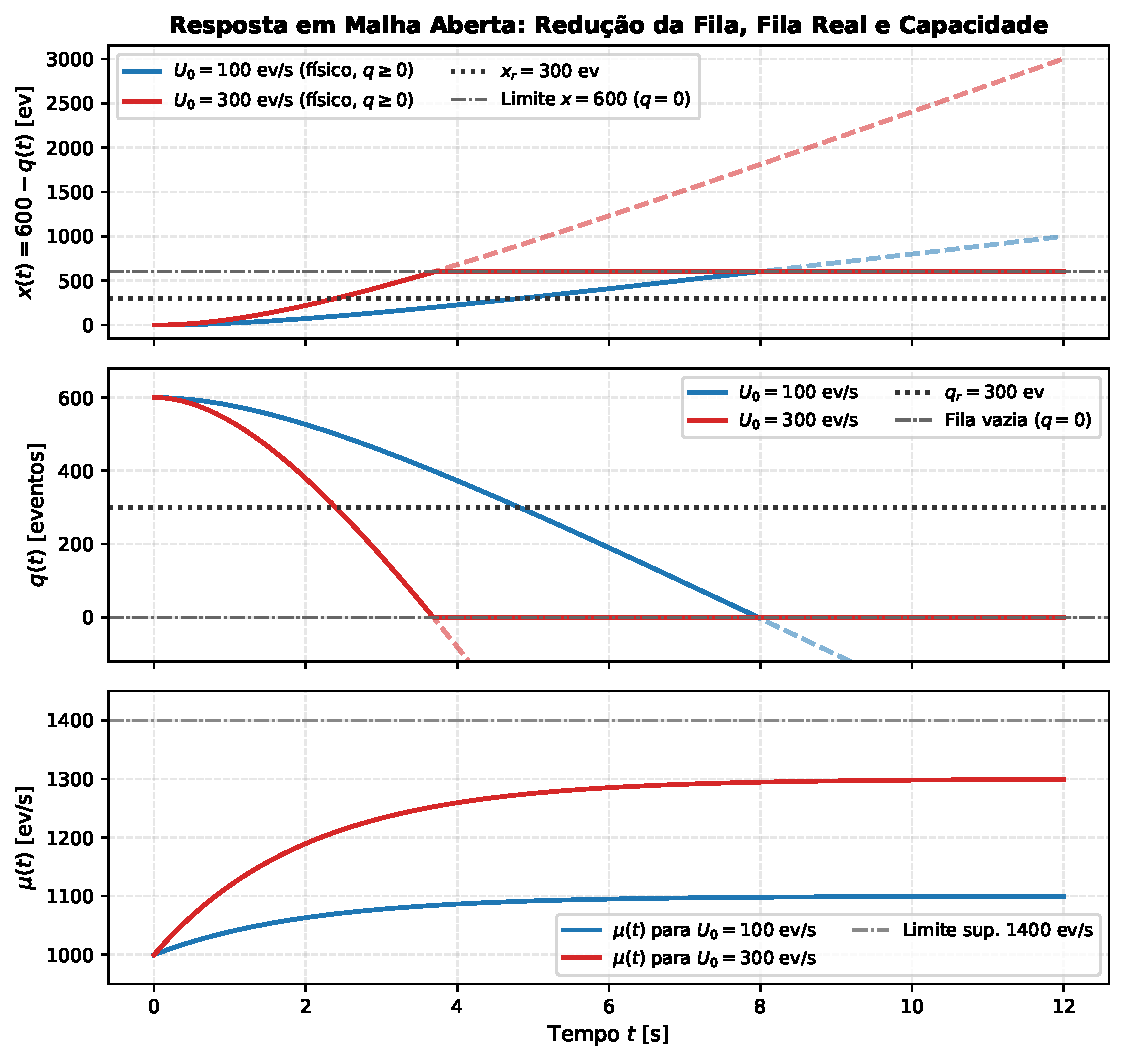
\includegraphics[width=0.74\textwidth]{figuras/fig1_malha_aberta.pdf}%
    }{%
        \fbox{\parbox{0.80\textwidth}{\centering\vspace{1.0cm}\textit{[Aguardando \texttt{figuras/fig1\_malha\_aberta.pdf}]}\vspace{1.0cm}}}%
    }
    \fontefig{Fonte: Elaborada pelos autores com base nos resultados de simulação (2026).}
\end{figure}
